\chapter{机器人的控制}
\label{ch:robot-control}

\begin{focusbox}{复习重点}
会从电枢电压与机械力矩平衡写出单关节传递函数，按特征方程选取位置和速度增益；会从动力学方程推出计算力矩、关节和笛卡尔阻抗，以及力/位混合控制。做接触控制题时，先选约束坐标系、画出力方向，再写控制律。PID 仿真、上述控制器设计和两种视觉伺服的比较见\hyperref[hw:robot-control]{控制部分课后作业精解}。
\end{focusbox}

\section{单关节电机建模与位置反馈}

\subsection{传动折算与开环模型}
取讲义的传动比约定 $n=z_m/z_L=\theta_L/\theta_m$，减速时 $0<n<1$。若设备铭牌把减速比写为 $i=\theta_m/\theta_L$，则 $n=1/i$；第\ref{chap:actuators}章用 $N=1/n$。由动能 $\tfrac12J_L\dot\theta_L^2=\tfrac12n^2J_L\dot\theta_m^2$ 和黏性耗散的同类关系，电机轴上的等效量为
\[
J_{\mathrm{eff}}=J_m+n^2J_L,\qquad f_{\mathrm{eff}}=f_m+n^2f_L.
\]
理想传动下 $\tau_m\dot\theta_m=\tau_L\dot\theta_L$，所以负载力矩折算到电机侧乘 $n$，负载惯量折算乘 $n^2$。例：$J_m=0.01\,\mathrm{kg\,m^2}$、$J_L=2\sim8\,\mathrm{kg\,m^2}$、$n=1/40$，则 $J_{\mathrm{eff}}=0.01125\sim0.015\,\mathrm{kg\,m^2}$（讲义第12页）。

令 $u_a,i_a,R_a,L_a$ 分别为电枢电压、电流、电阻、电感，$k_a$ 为力矩系数，$k_b$ 为反电势系数。把阻碍正转的扰动在电机侧记为 $d_m$，方程为
\[
\begin{aligned}
 u_a &= R_a i_a+L_a\dot i_a+k_b\dot\theta_m,\\
 J_{\mathrm{eff}}\ddot\theta_m+f_{\mathrm{eff}}\dot\theta_m &=k_ai_a-d_m,\qquad \theta_L=n\theta_m.
\end{aligned}
\]
令 $d_m=0$，在零初值下消去 $I_a$，得到负载角位移的开环模型
\[
G(s)=\frac{\Theta_L(s)}{U_a(s)}
 =\frac{n k_a}{s[(R_a+L_a s)(J_{\mathrm{eff}}s+f_{\mathrm{eff}})+k_a k_b]}.
\]
当电气动态远快于机械动态时，可令 $L_a\approx0$。定义 $\gamma=R_a f_{\mathrm{eff}}+k_a k_b$，简化为 $G(s)=n k_a/[s(R_a J_{\mathrm{eff}}s+\gamma)]$。若输出取角速度，则分子多乘一个 $s$。反电势使 $\gamma$ 中多出 $k_a k_b$，它与机械黏性项共同提供速度阻尼。

\subsection{闭环传递函数、阻尼与稳态误差}
以 $r=\theta_L^d$、$e=r-\theta_L$，按讲义用 $u_a=(k_p e+k_v\dot e)/n$。接回 $\Theta_L=GU_a$，得到
\[
\frac{\Theta_L(s)}{R(s)}=\frac{k_a(k_p+k_vs)}{D(s)},\qquad
D(s)=R_aJ_{\mathrm{eff}}s^2+(\gamma+k_ak_v)s+k_ak_p.
\]
\begin{figure}[H]
    \centering
    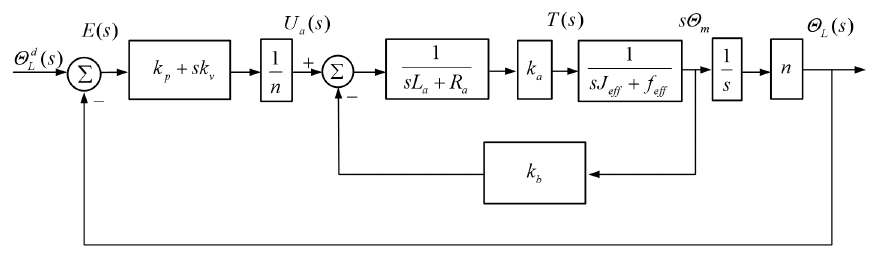
\includegraphics[width=0.95\linewidth]{05-joint-feedback.png}
    \caption{单关节位置、速度误差反馈及电机反电势内反馈。截取自第5章讲义 PDF 第17页。}
\end{figure}
比较 $D(s)/(R_aJ_{\mathrm{eff}})=s^2+2\zeta\omega_n s+\omega_n^2$ 各项系数得
\[
  \omega_n=\sqrt{\frac{k_a k_p}{R_aJ_{\mathrm{eff}}}},\qquad
  \zeta=\frac{\gamma+k_a k_v}{2\sqrt{R_aJ_{\mathrm{eff}}k_a k_p}}.
\]
给定 $\omega_n,\zeta$，先求 $k_p=R_aJ_{\mathrm{eff}}\omega_n^2/k_a$，再求 $k_v=(2\zeta\omega_n R_aJ_{\mathrm{eff}}-\gamma)/k_a$。$\zeta=1$ 时特征根重合，$0<\zeta<1$ 为欠阻尼，$\zeta>1$ 为过阻尼。读阶跃曲线还需看传递函数的零点，例如误差微分会在分子引入 $k_vs$，阶跃参考同时带来理想微分冲击。用 $u_a=[k_p(r-\theta_L)-k_v\dot\theta_L]/n$，分母相同、分子只有 $k_a k_p$。讲义用 $\omega_n\leq\omega_r/2$ 作避开结构共振的设计约束，$\omega_r$ 为结构共振频率。

用 $L_a=0$ 的模型保留 $d_m$，有 $D(s)\Theta_L=k_a(k_p+k_vs)R-nR_aD_m$，所以
\[
 E(s)=\frac{(R_aJ_{\mathrm{eff}}s^2+\gamma s)R(s)+nR_aD_m(s)}{D(s)}.
\]
闭环稳定时，对阶跃参考 $R=A/s$ 及恒定阻力矩 $D_m=d_0/s$，终值定理给出 $e_{\mathrm{ss}}=nR_a d_0/(k_a k_p)$。若 $d_0=0$，单位负反馈的角位置开环有一个积分环节，阶跃参考无静差。斜率为 $A$ 的斜坡参考 $R=A/s^2$ 则另有跟踪滞后 $A\gamma/(k_a k_p)$（采用误差微分）。重力等已知力矩可在电机侧前馈补偿，剩余扰动决定相应的静差。

\ex{按二阶极点选伺服增益}{若 $R_a=2$、$J_{\mathrm{eff}}=0.02$、$\gamma=0.11$、$k_a=0.1$，取 $\omega_n=4\,\mathrm{rad/s}$、$\zeta=1$，则 $k_p=0.04\times16/0.1=6.4$，$k_v=(0.04\times8-0.11)/0.1=2.1$。特征多项式变为 $s^2+8s+16=(s+4)^2$。只取 $k_p$ 时阻尼比为 $0.11/0.32\approx0.344$，增加速度反馈在模型中补足了阻尼。}

\section{控制规律分解与计算力矩}
\label{sec:computed-torque}
单轴模型 $m\ddot x+b\dot x+kx=f$ 有两种解法。直接按位移、速度反馈 $f=-k_px-k_v\dot x$，闭环的实际阻尼和刚度为 $b+k_v$、$k+k_p$。采用 $f=\alpha u+\beta$ 时，选 $\alpha=m,\ \beta=b\dot x+kx$ 得 $\ddot x=u$。令 $e=x_d-x$，用 $u=\ddot x_d+k_v\dot e+k_pe$ 即得 $\ddot e+k_v\dot e+k_p e=0$。在后一种写法中，$k_p=\omega_n^2$ 是归一化系数，定点附近抵抗外力的实际刚度为 $m k_p$。

多关节机械臂写作 $M(q)\ddot q+h(q,\dot q)=\tau$，其中 $M$ 是对称正定的惯性矩阵，$h$ 汇总科氏力、离心力、重力与摩擦等模型项。令 $e=q_d-q$，计算力矩法用
\[
\begin{aligned}
 u&=\ddot q_d+K_v\dot e+K_pe,\\
 \tau&=\widehat M(q)u+\widehat h(q,\dot q).
\end{aligned}
\]
帽号表示计算使用的模型。模型精确且无外扰时 $\ddot q=u$，所以 $\ddot e+K_v\dot e+K_pe=0$；取正对角增益，各轴化为独立的二阶误差系统，可令 $k_{p,i}=\omega_{n,i}^2$、$k_{v,i}=2\zeta_i\omega_{n,i}$。参考加速度提供前馈，误差反馈校正初始偏差与模型残差。模型参数不准时，剩余项随构型和速度变化，各轴可能再次耦合。

\section{约束坐标系与直接力控制}
\label{sec:force-control}
\dfn{自然约束与人工约束}{几何接触限制运动，环境也限制可传递的力，这些由环境决定，称为自然约束。人工约束指定机器人还可选择的量，例如沿光滑台面切向走给定轨迹、沿台面法向维持给定压力。约束坐标系以环境几何或任务方向选轴，可固定在环境中，也可随任务更新。}

\begin{figure}[H]
    \centering
    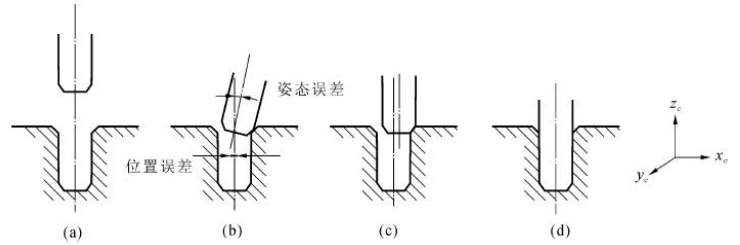
\includegraphics[width=0.76\linewidth]{05-peg-in-hole.png}
    \caption{圆棒入孔的接近、接触、对准、插入四个阶段。接触状态改变时，应重判自由方向与受约束方向。截取自第5章讲义 PDF 第47页。}
\end{figure}

单轴直接力控制以弹性接触为例。取压入为正，$f_e=k_e x$ 是机器人施于环境的力，$f$ 为驱动作用，$f_{\mathrm{dis}}$ 为额外阻力。由 $m\ddot x=f-f_e-f_{\mathrm{dis}}$ 得
\[
  f=\frac{m}{k_e}\ddot f_e+f_e+f_{\mathrm{dis}}\quad(k_e>0).
\]
以 $e_f=f_d-f_e$，取 $u_f=\ddot f_d+k_{vf}\dot e_f+k_{pf}e_f$，可以用 $f=(m/k_e)u_f+f_e$ 补偿接触弹力，或用 $f=(m/k_e)u_f+f_d$ 作参考力前馈。第一种误差方程为 $\ddot e_f+k_{vf}\dot e_f+k_{pf}e_f=(k_e/m)f_{\mathrm{dis}}$；第二种把刚度项系数改为 $k_{pf}+k_e/m$。常值扰动下，在闭环稳定时，后者稳态误差为 $f_{\mathrm{dis}}/(1+mk_{pf}/k_e)$。这两种式子只适用于接触模型成立的阶段，推导与增益选择见\hyperref[hw:control-10-3]{教材题 10.3}。

\section{顺应、阻抗与导纳}
\label{sec:robot-impedance}
\dfn{顺应与阻抗}{顺应描述外力引起的位移变化。被动顺应靠机械柔性，例如远中心柔顺装置 RCC 帮助插装对准；主动顺应通过控制设定刚度。阻抗在弹簧项之外还规定惯性和阻尼，描述交互的动态过程。}
局部小位移下 $\delta x=J\delta q$，由虚功 $f^{\mathsf T}\delta x=\tau^{\mathsf T}\delta q$ 得 $\tau=J^{\mathsf T}f$。因此定点无预载（或冻结 $J$）时，末端刚度 $K_x$ 对应的关节空间增量刚度为 $K_q=J^{\mathsf T}K_xJ$。接触通常取较低法向刚度缓冲碰撞，保留合适的切向刚度以跟踪轨迹。

\begin{figure}[H]
    \centering
    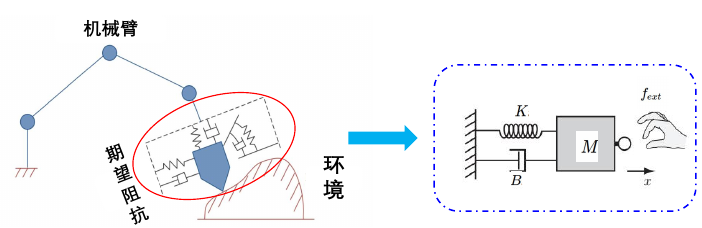
\includegraphics[width=0.79\linewidth]{05-impedance-model.png}
    \caption{用虚拟质量、阻尼和弹簧描述末端与环境的交互。截取自第5章讲义 PDF 第69页。}
\end{figure}
令 $\Delta x=x-x_d$，$f_{\mathrm{ext}}$ 为环境施于机器人的外力，典型目标模型为
\[
  M_d\Delta\ddot x+B_d\Delta\dot x+K_d\Delta x=f_{\mathrm{ext}}.
\]
$M_d,B_d,K_d$ 分别为期望惯量、阻尼、刚度，通常选为正定矩阵。若题目用 $e_x=x_d-x$，上式右端随之改为 $-f_{\mathrm{ext}}$。令 $Z_x(s)=F_{\mathrm{ext}}(s)/\Delta X(s)=M_d s^2+B_d s+K_d$（零初值），即讲义按位移定义的阻抗，也称动态刚度；按速度定义的机械阻抗为 $Z_x(s)/s$。单轴恒力平衡位移为 $f_{\mathrm{ext}}/K_d$，$M_d$ 和 $B_d$ 在此平衡式中消失。单轴瞬态的 $\omega_n=\sqrt{K_d/M_d}$、$\zeta=B_d/(2\sqrt{M_dK_d})$ 可用来设计过渡过程。

\begin{center}
\small
\begin{tabularx}{\linewidth}{@{}p{0.16\linewidth}XX@{}}
\toprule
控制方式 & 从测量到指令 & 总体实现 \\
\midrule
阻抗控制 & 位姿偏差、速度等 $\to$ 调节作用力/力矩 & 常与力矩或电流内环配合 \\
导纳控制 & 外力或力误差 $\to$ 通过二阶模型生成运动修正 & 常与位置或速度内环配合 \\
\bottomrule
\end{tabularx}
\end{center}
若对虚拟阻抗模型求逆，就有 $\Delta X=Z_x^{-1}F_{\mathrm{ext}}$。导纳实现将该二阶方程积分，得到运动参考供内环跟踪。关节空间把 $x,f_{\mathrm{ext}}$ 换为 $q,\tau_{\mathrm{ext}}$；笛卡尔空间还需用 $\dot x=J\dot q$、$\ddot x=J\ddot q+\dot J\dot q$ 或任务空间逆动力学。具体推导见\hyperref[hw:control-3]{作业第3题}。

\section{直接力/位置混合控制}
\label{sec:robot-hybrid}
在约束坐标系中选 $S_p$ 投影到位置控制方向。使用正交轴时，$S_p$ 为对角选择矩阵，位置轴取 $1$，余项取 $0$。力方向用 $S_f=I-S_p$，有 $S_pS_f=0$。在同一坐标系、同一广义量中合成命令，例如均写为笛卡尔广义力时
\[
 F_{\mathrm{cmd}}=S_p F_{\mathrm{pos}}+S_f F_{\mathrm{force}},\qquad
 \tau_{\mathrm{cmd}}=J_c^{\mathsf T} F_{\mathrm{cmd}}+\tau_{\mathrm{model}}.
\]
$J_c$ 将关节速度映射到该约束坐标系中的末端速度。上式给出信号分配，动力学耦合须由模型补偿或在控制器中考虑。纯位置控制的极端情形是 $S_p=I$；光滑台面接触中，约束系的两个切向分量由位置支路控制，法向分量由力支路控制。讲义例以 $y$ 为法向，则 $S_p=\operatorname{diag}(1,0,1)$，$S_f=\operatorname{diag}(0,1,0)$。位置矢量与力矢量须统一表达在约束系并分别形成误差，混合时再把换算后的同类指令相加。

\nt{自然约束与控制目标成对出现。光滑面切向不能承担理想摩擦力，可沿切向跟踪位置；法向运动受阻，可控制压力。接近接触点时先执行自由空间轨迹，确认建立接触后再启用法向力支路。}

\section{视觉伺服：从视觉特征误差生成运动}
\label{sec:visual-servo}
视觉伺服反复采集图像、估计误差并下发相机或机械臂速度。PBVS（基于位置）用从图像重建的三维相对位姿构造误差。IBVS（基于图像）用像点、线或其他图像特征构造误差。两者都是图像进入反馈环，差别在反馈误差所在的空间。

用相机速度旋量 $v_c=(v_x,v_y,v_z,\omega_x,\omega_y,\omega_z)^{\mathsf T}$，特征运动为 $\dot s=L_s v_c$，$L_s$ 称为交互矩阵。常用速度律 $v_c=-\lambda\widehat L_s^+(s-s_d)$，其中 $+$ 表示伪逆。若交互矩阵精确且在目标附近具有足够的秩，特征误差沿可控方向衰减。手眼结构还需将相机速度变换到机器人控制坐标系，再用机器人雅可比求关节速度。点特征的交互矩阵和 PBVS/IBVS 的优缺点见\hyperref[hw:control-5]{作业第5题}。

\section{考前自测}
\qs{控制模型与符号}{\begin{enumerate}
  \item 如果把传动比改记为 $i=40$，如何将负载惯量、负载力矩折算到电机轴？
  \item 位置误差微分与角速度负反馈的闭环特征多项式相同。为什么两者的阶跃响应仍可能不同？
  \item 目标误差定义从 $x-x_d$ 改成 $x_d-x$，外力方向保持原约定，阻抗等式应如何改写？
  \item 机器人沿无摩擦斜面滑动并保持法向压力，应如何写选择矩阵？
\end{enumerate}}
\noindent\textbf{核对}　(1) 分别除以 $i^2$、$i$。(2) 参考的微分通道改变分子，引入零点；理想阶跃会产生微分冲击。(3) 右端变为 $-f_{\mathrm{ext}}$。(4) 在法向为第三轴的约束系中，$S_p=\operatorname{diag}(1,1,0)$，$S_f=\operatorname{diag}(0,0,1)$。
